% =====================================================================
% The leakage-free splitting procedure. This is the original diagram from
% our weapon-detection paper (Catargiu & Ciocoiu, IEEE Access 2026),
% extracted from the published PDF. The procedure shown is the one applied
% unchanged to LuggageDataset v6i; the illustrative counts printed inside
% the panels are from the weapon corpus and are restated for v6i in the
% caption and in the accompanying text.
% =====================================================================
\begin{figure*}[t]
\centering
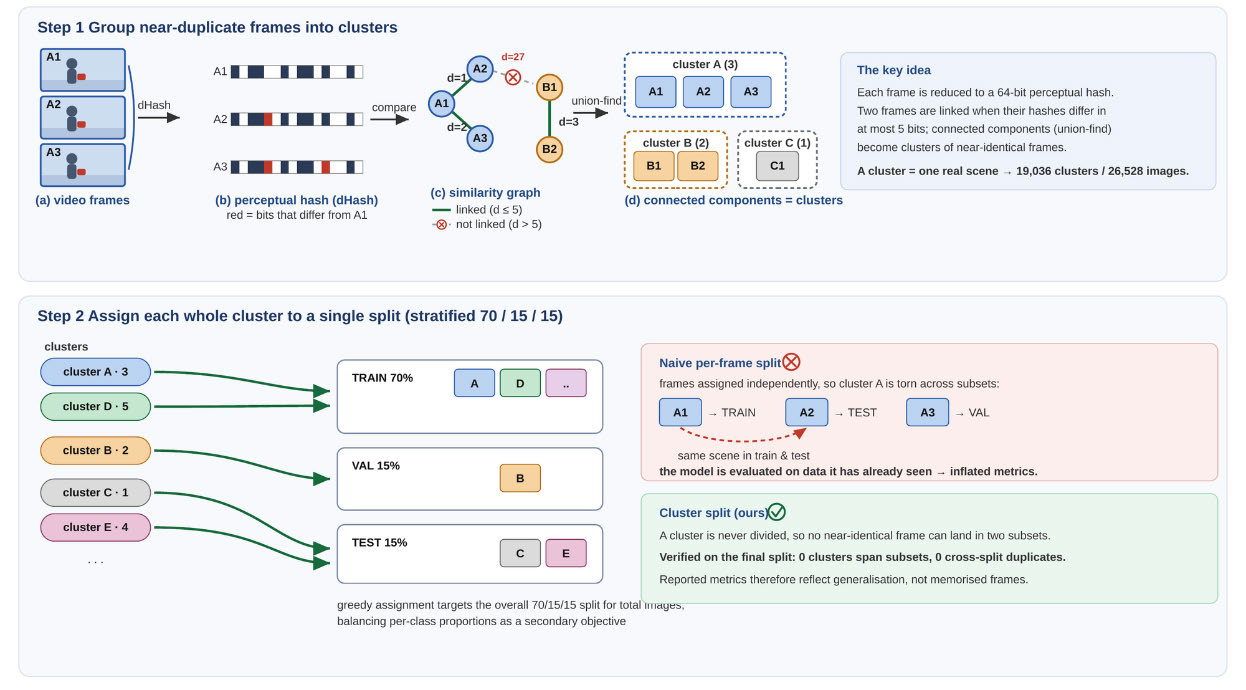
\includegraphics[width=\linewidth]{fig_leakage.png}
\caption{The leakage-free splitting procedure. \textbf{Step 1:} each frame is
reduced to a 64-bit perceptual (difference) hash; any two frames whose hashes
differ in at most five bits are linked, and connected components extracted by
union-find group mutually near-identical frames into clusters, so that one
cluster corresponds to one real scene. \textbf{Step 2:} each whole cluster,
never an individual frame, is assigned to a single split by a stratified greedy
procedure, so no near-duplicate frame can cross a split boundary by
construction. The panels illustrate the method with the counts from the
weapon-detection corpus in which it was first validated
\cite{catargiu2026weapon}; applied unchanged to LuggageDataset~v6i at the same
Hamming threshold of five, it produces the $75/15/10$ partition of
Table~\ref{tab:splits} and a cross-split audit of that partition returns
\textbf{zero} clusters spanning subsets and \textbf{zero} near-duplicate pairs
between any two subsets.}
\label{fig:leakage}
\end{figure*}
